\documentclass[12pt]{scrartcl}
\usepackage{graphicx}
\usepackage{amsmath}

\begin{document}

%Title section

\titlehead{CS department, Technion}
\subject{Introduction to Optimization and Deep Learning 236330}
\title{HW 3}
\subtitle{Quasi-Newton BFGS method and DNN training}
\author{Uri Kirstein 311137095 \hfill sukirstn@campus.technion.ac.il\and Pavel Rastopchin 321082026 pavelr@campus.technion.ac.il}
\date{\today}
\maketitle

 %end of title section
\section*{Part 1 - BFGS}
\subsection*{Task 2}
We chose $N=10$. Our starting point was $x_0=(0,0,..0)$. We know that a local minimum of the function exists at $x^*=(1,1,...)$ and that $p^*=0$ (our function is non-negative so this must be a global minimum as well). We stopped after 60 iterations (we started from iteration number 0) at
\begin{center}
$x_{final}$ =[ 1.,  1., 1., 1., 1., 1., 1., 1., 1., 1.]
\end{center}
The error function and gradient at this point is $$f(x_{final})-p^*\approx 0$$
$\nabla f(x_{final})=$[-1.03489194e-07 4.64227620e-07 -2.33440170e-07 -3.37145026e-07 \\
4.63302603e-07 1.27499791e-07 -6.70338432e-07 5.13097599e-07 -3.48798911e-07 \\
1.10922516e-07]
$$||\nabla f(x_{final})|| = 1.2132069569224647e-06$$
We can see in the graph below that the error function $f(x_k)-p^*$, where $k$ is the number of iterations, is monotonously decreasing. This means we always advance in the direction of the minimum.
\begin{figure}[ht!]
	\hfill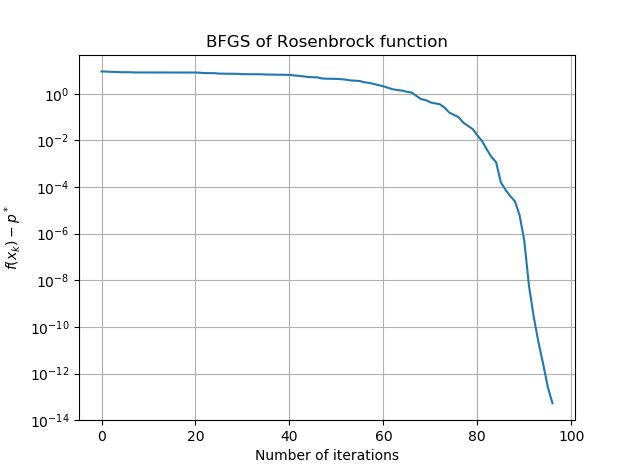
\includegraphics[width=\linewidth]{rosenbrock_graph.jpg}\hspace*{\fill}
	\caption{Task 2}
\end{figure}

\section*{Part 2 - Deep Neural Network}
\subsection*{Task 3}
\begin{align*}
\Psi(r_i)&=r_i^2\\
&=[F(x^i,w)-y_i]^2\\
&=\{w_3^T\varphi_2[w_2^T\varphi_1(w_1^Tx^i+b_1)+b_2]+b_3 -x_1^i exp[-(x_1^i)^2-(x_2^i)^2]\}^2
\end{align*}
We will use the following derivative:
$$\frac{d}{dx}\varphi_1=\frac{d}{dx}\varphi_2=\frac{d}{dx}tanh(x)=
\frac{1}{cosh^2(x)}$$

$$\Phi'(x)=
\begin{pmatrix}
\varphi'(x_1) & \cdots & 0 \\
\vdots & \ddots & \vdots \\
0 & \cdots & \varphi'(x_n)
\end{pmatrix}
=
\begin{pmatrix}
\frac{1}{cosh x_1} & \cdots & 0 \\
\vdots & \ddots & \vdots \\
0 & \cdots & \frac{1}{cosh x_n}
\end{pmatrix}$$

$$\nabla_r \Psi = 2r$$
$$\nabla_x \Psi = J^T_{F(x, W)}\nabla_r \Psi = 
W_1\Phi_1'W_2\Phi_2'W_3\nabla_r \Psi$$
As the gradient calculation is difficult, we will do it in steps. We will define the following middle points:
\begin{center}
$u_1 = W_1^Tx+b_1$, $u_2 = W_2^T\varphi(u_1)+b_2$, $u_3 = W_3^T\varphi(u_2)+b_3$
\end{center}
We can calculate their gradients
\begin{align*}
\nabla_{u_1} \Psi &= \Phi_1'W_2\Phi_2'W_3\nabla_r \Psi \\
\nabla_{u_2} \Psi &= \Phi_2'W_3\nabla_r \Psi \\
\nabla_{u_3} \Psi &= \nabla_r \Psi
\end{align*}

Now we can calculate the gradients with respect to the weights and bias parameters.

%gradient by w1
\begin{align*}
d\Psi &= \nabla_{u_1}\Psi^Tdu_1=\nabla_{u_1}\Psi^T dW_1^Tx
=Tr(\nabla_{u_1}\Psi^T dW_1^Tx)=Tr(x\nabla_{u_1}\Psi^T dW_1^T)
=x\nabla_{u_1}\Psi^T dW_1^T\\
d\Psi &= \nabla_{u_1}\Psi x^TdW_1 
\end{align*}
$\Rightarrow \nabla_{W_1}\Psi = \nabla_{u_1}\Psi x^T$
\begin{center}
\boxed{\nabla_{W_1}\Psi =  \Phi_1'W_2\Phi_2'W_3\nabla_r \Psi x^T}
\end{center}

%gradient by b1
$$d\Psi = \nabla_{u_1}\Psi^Tdu_1 = \nabla_{u_1}\Psi^T db_1 \Rightarrow \nabla_{b_1}\Psi = \nabla_{u_1} \Psi$$
\begin{center}
\boxed{\nabla_{b_1}\Psi = \Phi_1'W_2\Phi_2'W_3\nabla_r \Psi}
\end{center}

%gradient by w2
\begin{align*}
d\Psi &= \nabla_{u_2}\Psi^Tdu_2 = \nabla_{u_2}\Psi^T dW_2^T\varphi(u_1) = Tr(\nabla_{u_2}\Psi^T dW_2^T\varphi(u_1)) =
Tr(\varphi(u_1)\nabla_{u_2}\Psi^T dW_2^T)\\
&= \varphi(u_1)\nabla_{u_2}\Psi^T dW_2^T = \nabla_{u_2}\Psi\varphi(u_1)^T dW_2
\end{align*}
$\Rightarrow \nabla_{W_2}\Psi = \nabla_{u_2}\Psi\varphi(u_1)^T$
\begin{center}
\boxed{\nabla_{W_2}\Psi = \Phi_2'W_3\nabla_r \Psi \varphi(u_1)^T}
\end{center}

%gradient by b2
$$d\Psi = \nabla_{u_2}\Psi^Tdu_2 = \nabla_{u_2}\Psi^T db_2 \Rightarrow \nabla_{b_2}\Psi = \nabla_{u_2} \Psi$$
\begin{center}
\boxed{\nabla_{b_2}\Psi = \Phi_2'W_3\nabla_r \Psi}
\end{center}

%gradient by w3
\begin{align*}
d\Psi &= \nabla_{u_3}\Psi^Tdu_3 = \nabla_{u_3}\Psi^TdW_3^T\varphi(u_2) = Tr(\nabla_{u_3}\Psi^TdW_3^T\varphi(u_2))
= Tr(\varphi(u_2)\nabla_{u_3}\Psi^TdW_3^T)\\
&= \varphi(u_2)\nabla_{u_3}\Psi^TdW_3^T
= \nabla_{u_3}\Psi \varphi(u_2)^T dW_3
\end{align*}
$\Rightarrow \nabla_{u_3}\Psi = \nabla_{u_3}\Psi \varphi(u_2)^T$
\begin{center}
\boxed{\nabla_{W_3}\Psi = \nabla_r \Psi \varphi(u_2)^T}
\end{center}

%gradient by b3
$$d\Psi = \nabla_{u_3}\Psi^Tdu_3 = \nabla_{u_2}\Psi^T db_3 \Rightarrow \nabla_{b_3}\Psi = \nabla_{u_3} \Psi$$
\begin{center}
\boxed{\nabla_{b_3}\Psi = \nabla_r \Psi}
\end{center}


\end{document}
